%
% File naaclhlt2016.tex
%

\documentclass[11pt,letterpaper]{article}
\usepackage{naaclhlt2016}
\usepackage{times}
\usepackage{latexsym}
\usepackage{fancyvrb}
\usepackage{graphicx}
\usepackage[table,xcdraw]{xcolor}

\naaclfinalcopy % Uncomment this line for the final submission
\def\naaclpaperid{***} %  Enter the naacl Paper ID here

% To expand the titlebox for more authors, uncomment
% below and set accordingly.
% \addtolength\titlebox{.5in}    

\newcommand\BibTeX{B{\sc ib}\TeX}


\title{Translating Navigational Instructions in English to a Formal Representation}

% Author information can be set in various styles:
% For several authors from the same institution:
% \author{Author 1 \and ... \and Author n \\
%         Address line \\ ... \\ Address line}
% if the names do not fit well on one line use
%         Author 1 \\ {\bf Author 2} \\ ... \\ {\bf Author n} \\
% For authors from different institutions:
% \author{Author 1 \\ Address line \\  ... \\ Address line
%         \And  ... \And
%         Author n \\ Address line \\ ... \\ Address line}
% To start a seperate ``row'' of authors use \AND, as in
% \author{Author 1 \\ Address line \\  ... \\ Address line
%         \AND
%         Author 2 \\ Address line \\ ... \\ Address line \And
%         Author 3 \\ Address line \\ ... \\ Address line}
% If the title and author information does not fit in the area allocated,
% place \setlength\titlebox{<new height>} right after
% at the top, where <new height> can be something larger than 2.25in
\author{
    Vivin Suresh Paliath\\
    Arizona State University\\	    
    {\tt vivin.paliath@asu.edu>}
\And
    Vivek Patwari\\
    Arizona State University\\
    {\tt <vpatwar0@asu.edu>}
\AND    
    Anshul Tripathi\\
    Arizona State University\\
    {\tt <atripa10@asu.edu>}  
\And
    Aravinda Kumar Reddy Yempada\\
  	Arizona State University\\
    {\tt <ayempada@asu.edu>}
}

\date{November 30^{th}, 2015}

\begin{document}

\maketitle

\begin{abstract}
Computer-aided navigation is an indispensable part of modern-day life. However, the instructions provided by these systems are only as good as the underlying data; inaccurate or incomplete data limits the reliability of directions. While a human-being can then rely on ad hoc navigational instructions to find their way, it would be useful if a machine was able to do the same. However, the ambiguous and free-form nature of natural-language isn't suitable makes this difficult; a formal, unambiguous representation is required. In this paper, we propose a technique that uses CCG-based parsing and semantic learning (using inverse-lambda and generalization algorithms) to translate English-language navigational instructions to a formal form. We use NL2KR to learn the meanings of specific words and then translate them to a formal form. Evaluation was performed by comparing translated forms to their English-language counterparts, and also by creating a simulated environment with an agent capable of understanding the formal representation.
\end{abstract}

\section{Introduction}

Knowledge representation deals with representing information in a manner that a computer can analyze and utilize. There are many kinds of representations, each tailored towards solving different kinds of problems. In effect, they are domain-specific languages that have been designed to model a particular concept. Consider the implications of applying this technique to navigational instructions. If there was a formal representation of ad-hoc navigational instructions, it would be possible for a machine to follow those instructions to arrive at a destination. However, the usefulness of this approach is limited unless we provide a mapping from natural-language navigational-instructions to a formal representation. Due to the free-form nature of natural-languages, there are a multitude of ways a particular route or even part of a route can be described. For example, the route could simply use directions and units of distance, or it could use landmarks as points of reference. Manually mapping every-possible variation of navigational-instruction to a formal form would be time-consuming and a never-ending task for the most part. Instead, it would be far-more beneficial if the process could be automated such that the formal-representation can be derived automatically from the natural-language form.

In this paper, we propose such a method: we use CCG-based parsing along with semantic learning to convert English-language navigational-instructions into a formal form. Individual words and their meanings (in terms of the formal representation) are first defined using lambda-calculus expressions. In addition, the words are also tagged with their syntactic type. The system is also provided a set of English-language navigational-instructions and their equivalent formal-forms. Using this training data, the system parses the English-language sentences, and uses inverse-lambda and generalization algorithms against the CCG parse-tree to learn the meanings of new words. Weights are estimated for each word and its meaning using a parameter-learning method, to maximize the probability that the sentences in the training set match against the appropriate formal-representation. We then evaluate the performance of our method against a test set, and also by means of a simulation that involves a simple, two-dimensional grid inhabited by an agent capable of understanding the formal representation.

\section{Techniques used}

We use the NL2KR\cite{baral2013nl2kr} system (which uses the earlier-described techniques) to implement our approach. To construct our initial training set and to identify key-words we used an existing data-set of navigational instructions\cite{chen2011learning} to construct the lexicon. Subsequent sections will go over each component in greater detail.

\subsection{Formal representation}

\begin{figure}[ht!]
\begin{Verbatim}[fontfamily=courier,fontsize=\footnotesize,fontseries=b]

instructions ::= { instruction }
instruction  ::= start | turn | move | 
                 verify
start        ::= "start", "(", number,
                 ",", number, ")"
turn         ::= "turn", "(", 
                 ( direction | until ), 
                 ")"
direction    ::= relative | absolute
relative     ::= left | right | front |
                 back
absolute     ::= north | south | east | 
                 west
until        ::= "until", "(", conditions, 
                 ")"
conditions   ::= condition, { ",", 
                 condition }
condition    ::= "is", "(", object, 
                 [ ",", position ], ")"
object       ::= object-name, 
                 [ "(" attribute, 
                   { ",", attribute } 
                   ")" ]                   
attribute    ::= adjective | object
position     ::= "at", "(", orientation, 
                 ")"
orientation  ::= direction | 
                 [ direction, "," ], 
                 distance
distance     ::= unit, "(", number, ")"
move         ::= "move", "(", 
                 ( distance | until ), 
                 ")"
verify       ::= "verify", "(", that, ")"
that         ::= "that", "(", conditions,
                 ")"
\end{Verbatim}
\caption{EBNF for formal form}\label{fig:ebnf}
\end{figure}

Prior to training, we had to first define a formal representation that can adequately convey the semantics of navigational instructions in an unambiguous manner. The formal form that we eventually designed, defines simple primitives that can be combined to represent complex navigational-instructions. The EBNF for the formal form is shown in Figure~\ref{fig:ebnf}, and the instructions and their meanings are as follows:
\begin{itemize}
    \item \textbf{start}: Positions the agent on a two-dimensional grid. This is the only instruction that is tightly coupled to the simulation-environment, and it does not really have an equivalent in English.
    \item \textbf{turn}: Turns the agent. This instruction can take an absolute or relative direction (like "north" or "left"), or a reference point (e.g., "Turn until the yellow wall in on the left.").
    \item \textbf{move}: This moves the agent in the same direction as it is currently facing. It can take a distance (such as "5 spaces") or a reference point (e.g., "Move until the red door is in front of you.").
    \item \textbf{verify}: This statement verifies that the agent is at an expected location (e.g., "There should be an open window to the left.").
\end{itemize}

The form is expressive enough to encode instructions that use directions (both cardinal and relative), units of space, and reference-points and landmarks, yet is easily-parsable and is human-readable as well. For example, given the sentence:
\begin{quote}
\textit{Face away from the blue wall. Walk five steps and turn left. Keep going until you are in front of an old painting. Go away from the lamp until you are in front of a yellow door. There should now be a hallway with red carpet two spaces away on your left.}
\end{quote}

We can translate it to the formal-representation as seen in Figure~\ref{fig:formal}.
\begin{figure}
\begin{Verbatim}[fontfamily=courier,fontsize=\footnotesize,fontseries=b]
turn(until(is(wall(blue), at(back))))
move(steps(5))
turn(left)
move(until(
  is(painting(green), at(north)))
)
turn(until(is(lamp, at(south))))
move(until(is(door(yellow), at(front))))
verify(that(
  is(hallway(carpet(red)), 
     at(left, spaces(2)))
))
\end{Verbatim}
\caption{Formal representation of English navigational instructions}\label{fig:formal}
\end{figure}

\subsection{Using NL2KR}\label{ssec:usingnl2kr}

Having designed the formal representation, we started creating an initial lexicon of words and their meanings in lambda-calculus expressions, that used our formal form. We also manually created a small training-set using instructions from the existing data set. At this point we ran into a few issues that we had to resolve. First, we found that there were certain sentences that NL2KR was unable to parse (the parser would crash), which meant that we couldn't use any instructions of that particular variation. In addition, certain sentences didn't parse as expected according to the default syntax-file. Hence, we had to provide syntax overrides to ensure that the parse-trees had the structure that we wanted. However, as we started increasing the number of sentence variations and meanings, we noticed that we were unable to parse certain sentence-variations because that would require a different syntax-override that conflicted with an existing one. Furthermore, certain sentences would \textit{always} be parsed in a particular way \textit{regardless} of the syntax-override, since that particular parse tree was more probable than the one with the override.

We also faced some issues with the lambda syntax used by NL2KR which made it difficult to express associativity. Specifically, NL2KR treats two tokens separated by a comma as two separate tokens, and it is not possible to tell NL2KR to consider both of these as single argument to a function (there are ways around, but it involves the creation of a place-holder function). For example, assume that we need to group two arguments so that they can be represented as a pair of arguments to a function in the formal form. The token for that function will have to be associated with the meaning of one of the two words (i.e., the arguments), instead of being associated with a common ancestor. In spite of these stumbling blocks, we were still able to train 70 sentences and 103 meanings. In addition, we were also able to translate new sentences using the trained lexicon.

\subsection{Evaluation and Simulation}

Our initial strategy to evaluate our approach was manual: we would manually build up a test and training set (along with the equivalent formal-forms) and then compare the translated output. We initially took this approach because we were going to rely on the existing navigational data set. However, due to the issues encountered with NL2KR (as detailed in \S\ref{ssec:usingnl2kr}), we found that we couldn't rely on this strategy. Furthermore, we also realized that manual verification of the translation could be error-prone. Hence, we decided to use an approach similar to the one used by Chen et al., and developed a simulation of a world occupied by an agent (a robot) that is able to parse and understand the formal representation. The world is a two-dimensional grid with objects placed at different locations and also a path that the robot is able to navigate (see Figure~\ref{fig:navsim}).

\begin{figure}[h]
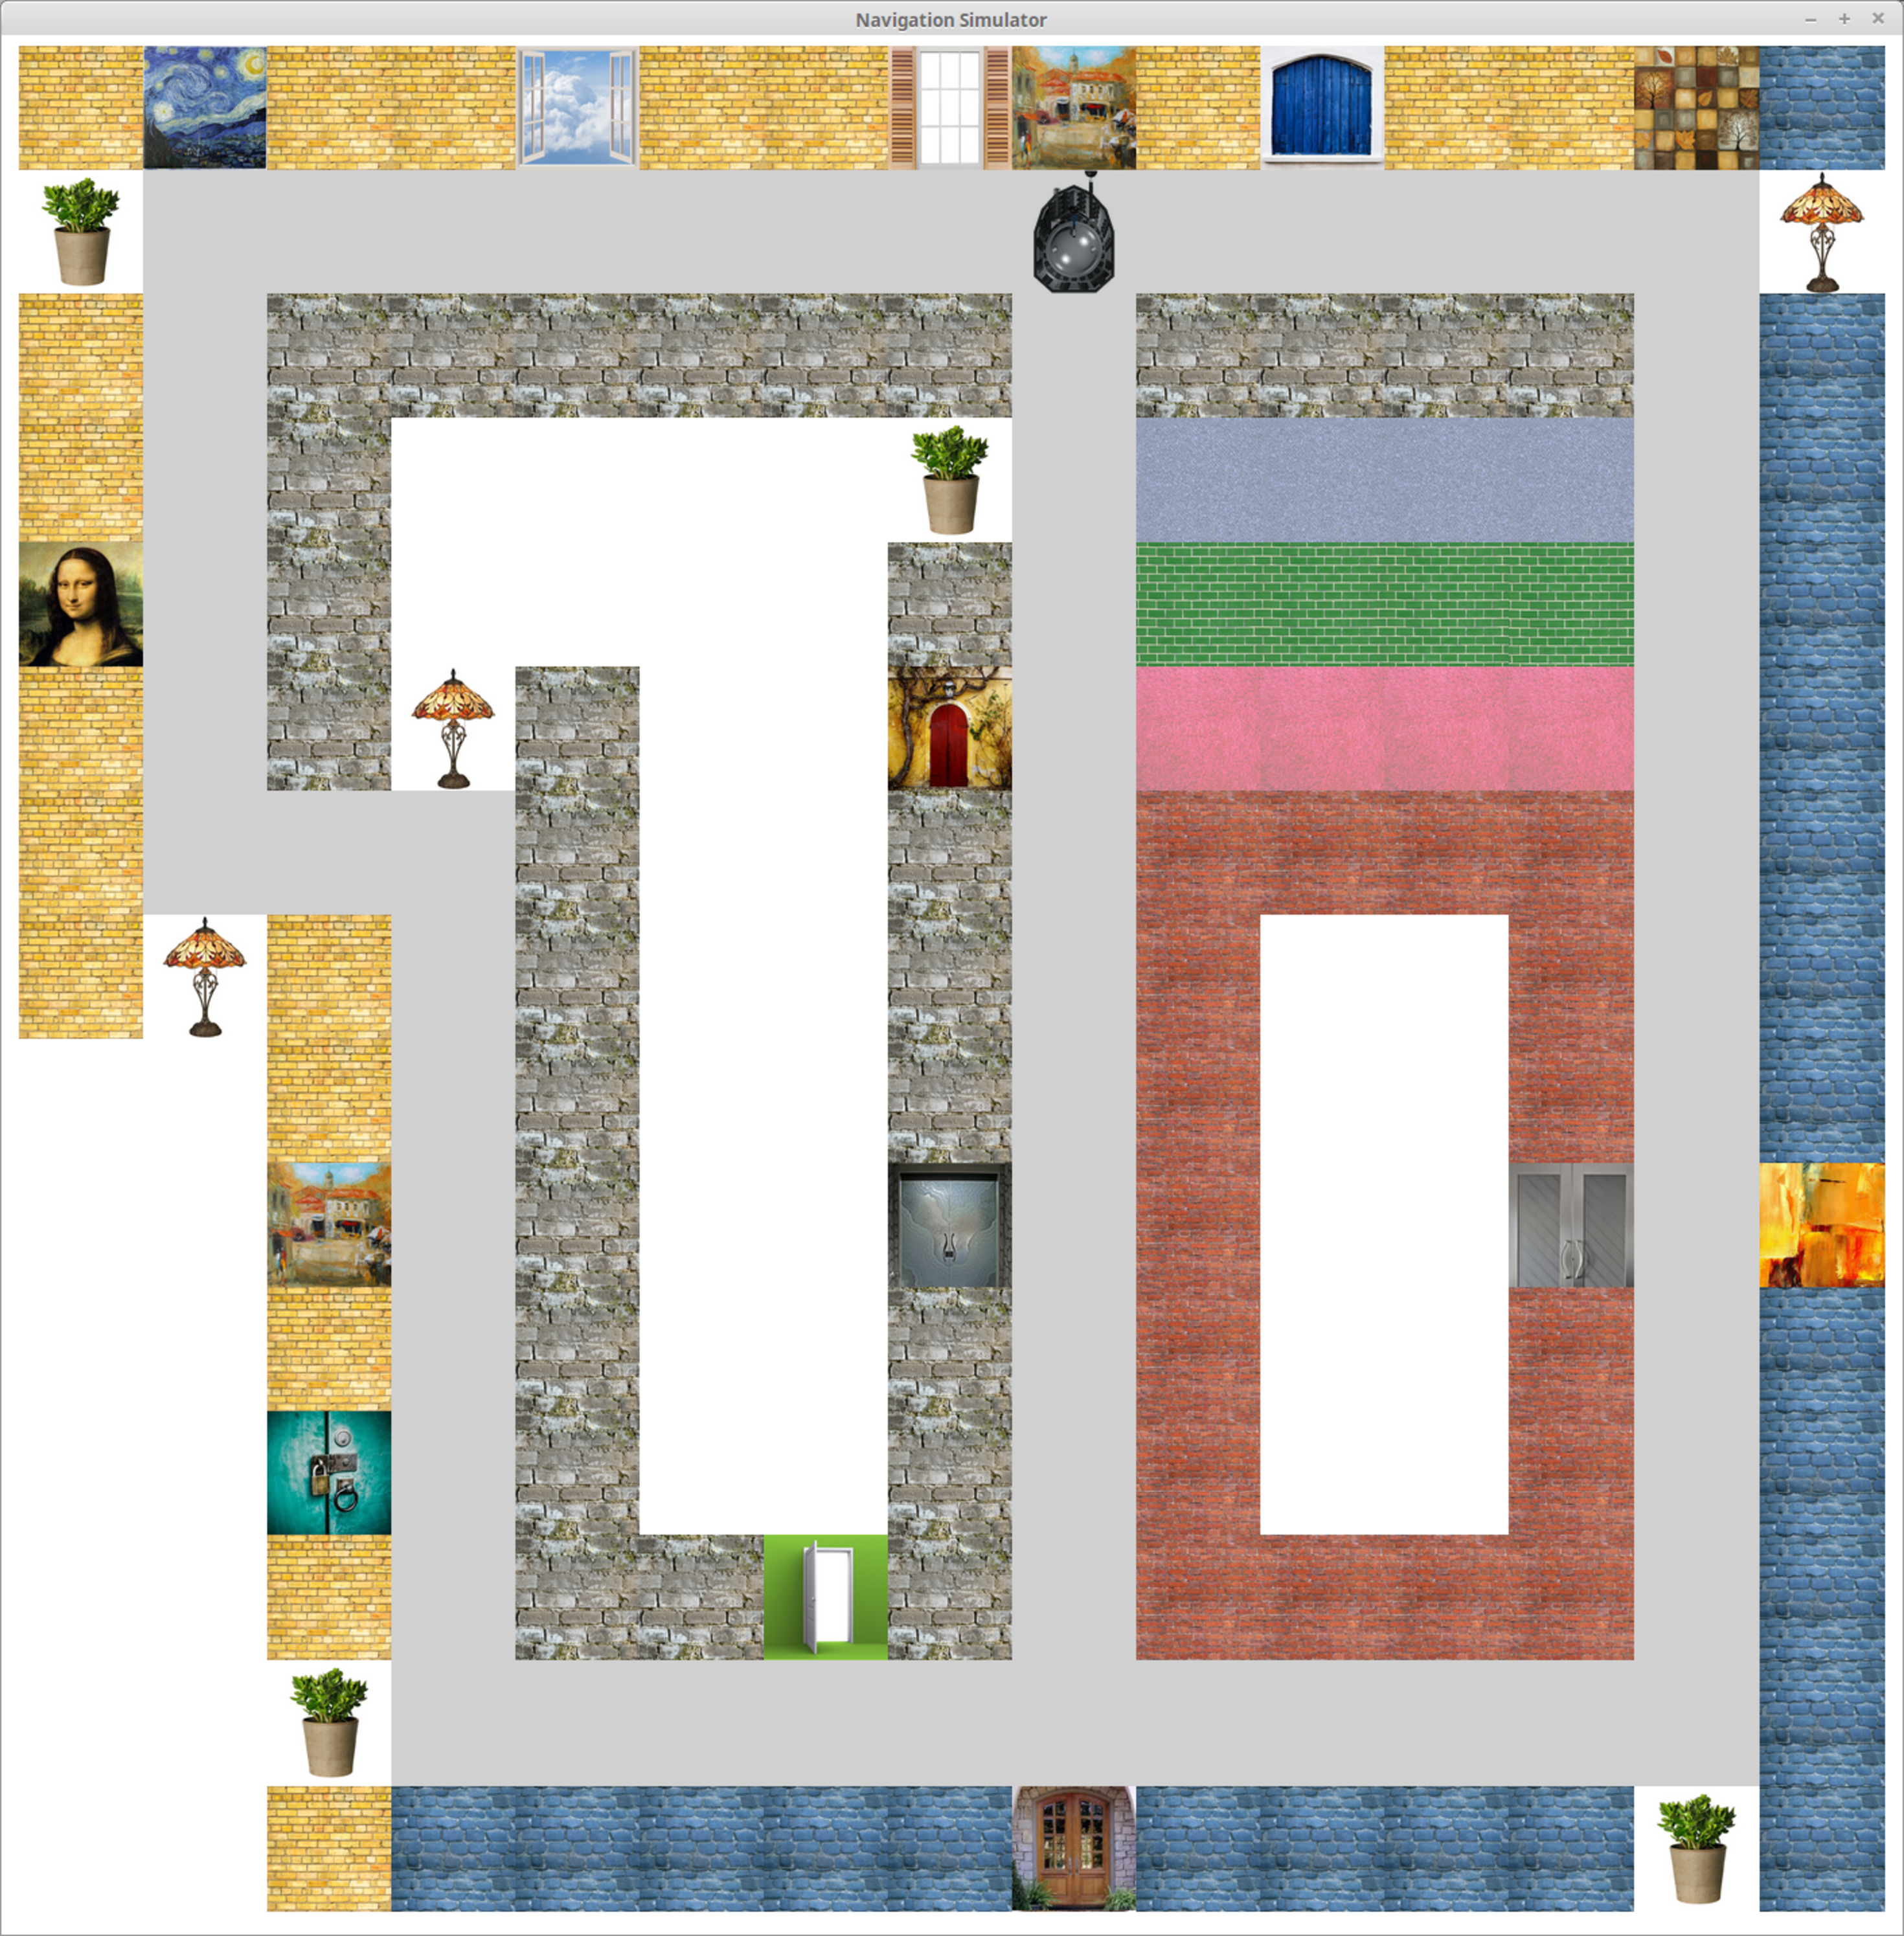
\includegraphics[scale=0.15]{navsim.pdf}
\caption{Navigation simulator showing simulated world with the robot at (12, 3)}\label{fig:navsim}
\end{figure}

\subsection{Simulation environment}

As mentioned earlier, the simulation environment is a two-dimensional grid with obstructions, objects, and paths. Every object in the world (except for grey paths and white spaces) has specific names and attributes. Individual locations in the world are identified using the row and the column. For example, in Figure~\ref{fig:navsim}, the robot is at row 12 and column 3.

The robot can perform turn and move actions in a way that is consistent with the formal representation. It understands explicit directions and distances, and so is able to turn to a particular direction or move a certain number of distances. The robot also has the ability to scan its immediate surroundings and everything in its line of sight. Using this information, it can perform more-complicated actions like turning until it is oriented a certain way with respect to a reference object (similar to a landmark), or moving until it detects a certain object. The robot can also scan its surroundings and verify that it is in a particular location based on the objects around it.

\subsection{Simulator and simulation process}

The simulator is a simple web-based application running on the node-webkit platform (also known as nwjs). The user interface was constructed using HTML5, and the simulator logic (including the parser for the formal form) was implemented in JavaScript. 

The simulator's user interface is quite simple (Figure~\ref{fig:interface}). The user can provide an English sentence, which is first translated using NL2KR into the formal form. This formal form is then provided to the robot, which parses it and converts it into an (internal) intermediate representation. Using this intermediate representation, it executes the provided instructions to the best of its ability. If the robot is unable to successfully execute any instruction, it will raise an error, which lets us know that the translation was not correct. For example, assume that the robot was asked to move until it encounters a red door on its left. The robot will move one step, and scan its surroundings to see if there is a red-door on its left. It will continue this process until the condition is satisfied, or until it cannot move any further. In the latter case, an error is raised. Similarly, if the robot is asked to face away from some object, it will continue to turn until that object is at its back. If it has turned a full circle without satisfying the condition, an error is raised as well. The robot verifies its destination in a manner quite similar to the move instruction, but with the added capability of being able to verify its location against distant landmarks (for example, an old painting that is two spaces away on the left). 

It is also possible to visually ascertain the accuracy of the translation by observing the actions taken by the robot. For example, let us assume that the robot is starting at location (13, 6) and is then issued a turn instruction (Figure~\ref{fig:turninst}). Figure~\ref{fig:robotturning} then shows the robot in the process of executing the turn instruction towards the correct direction. In Figure~\ref{fig:verifysuccess} and Figure~\ref{fig:verifyfail}, it is possible to see examples of a successful and unsuccessful verification instruction. In this manner, we can translate and verify that the translation is correct, quite quickly.

\begin{figure}[ht!]
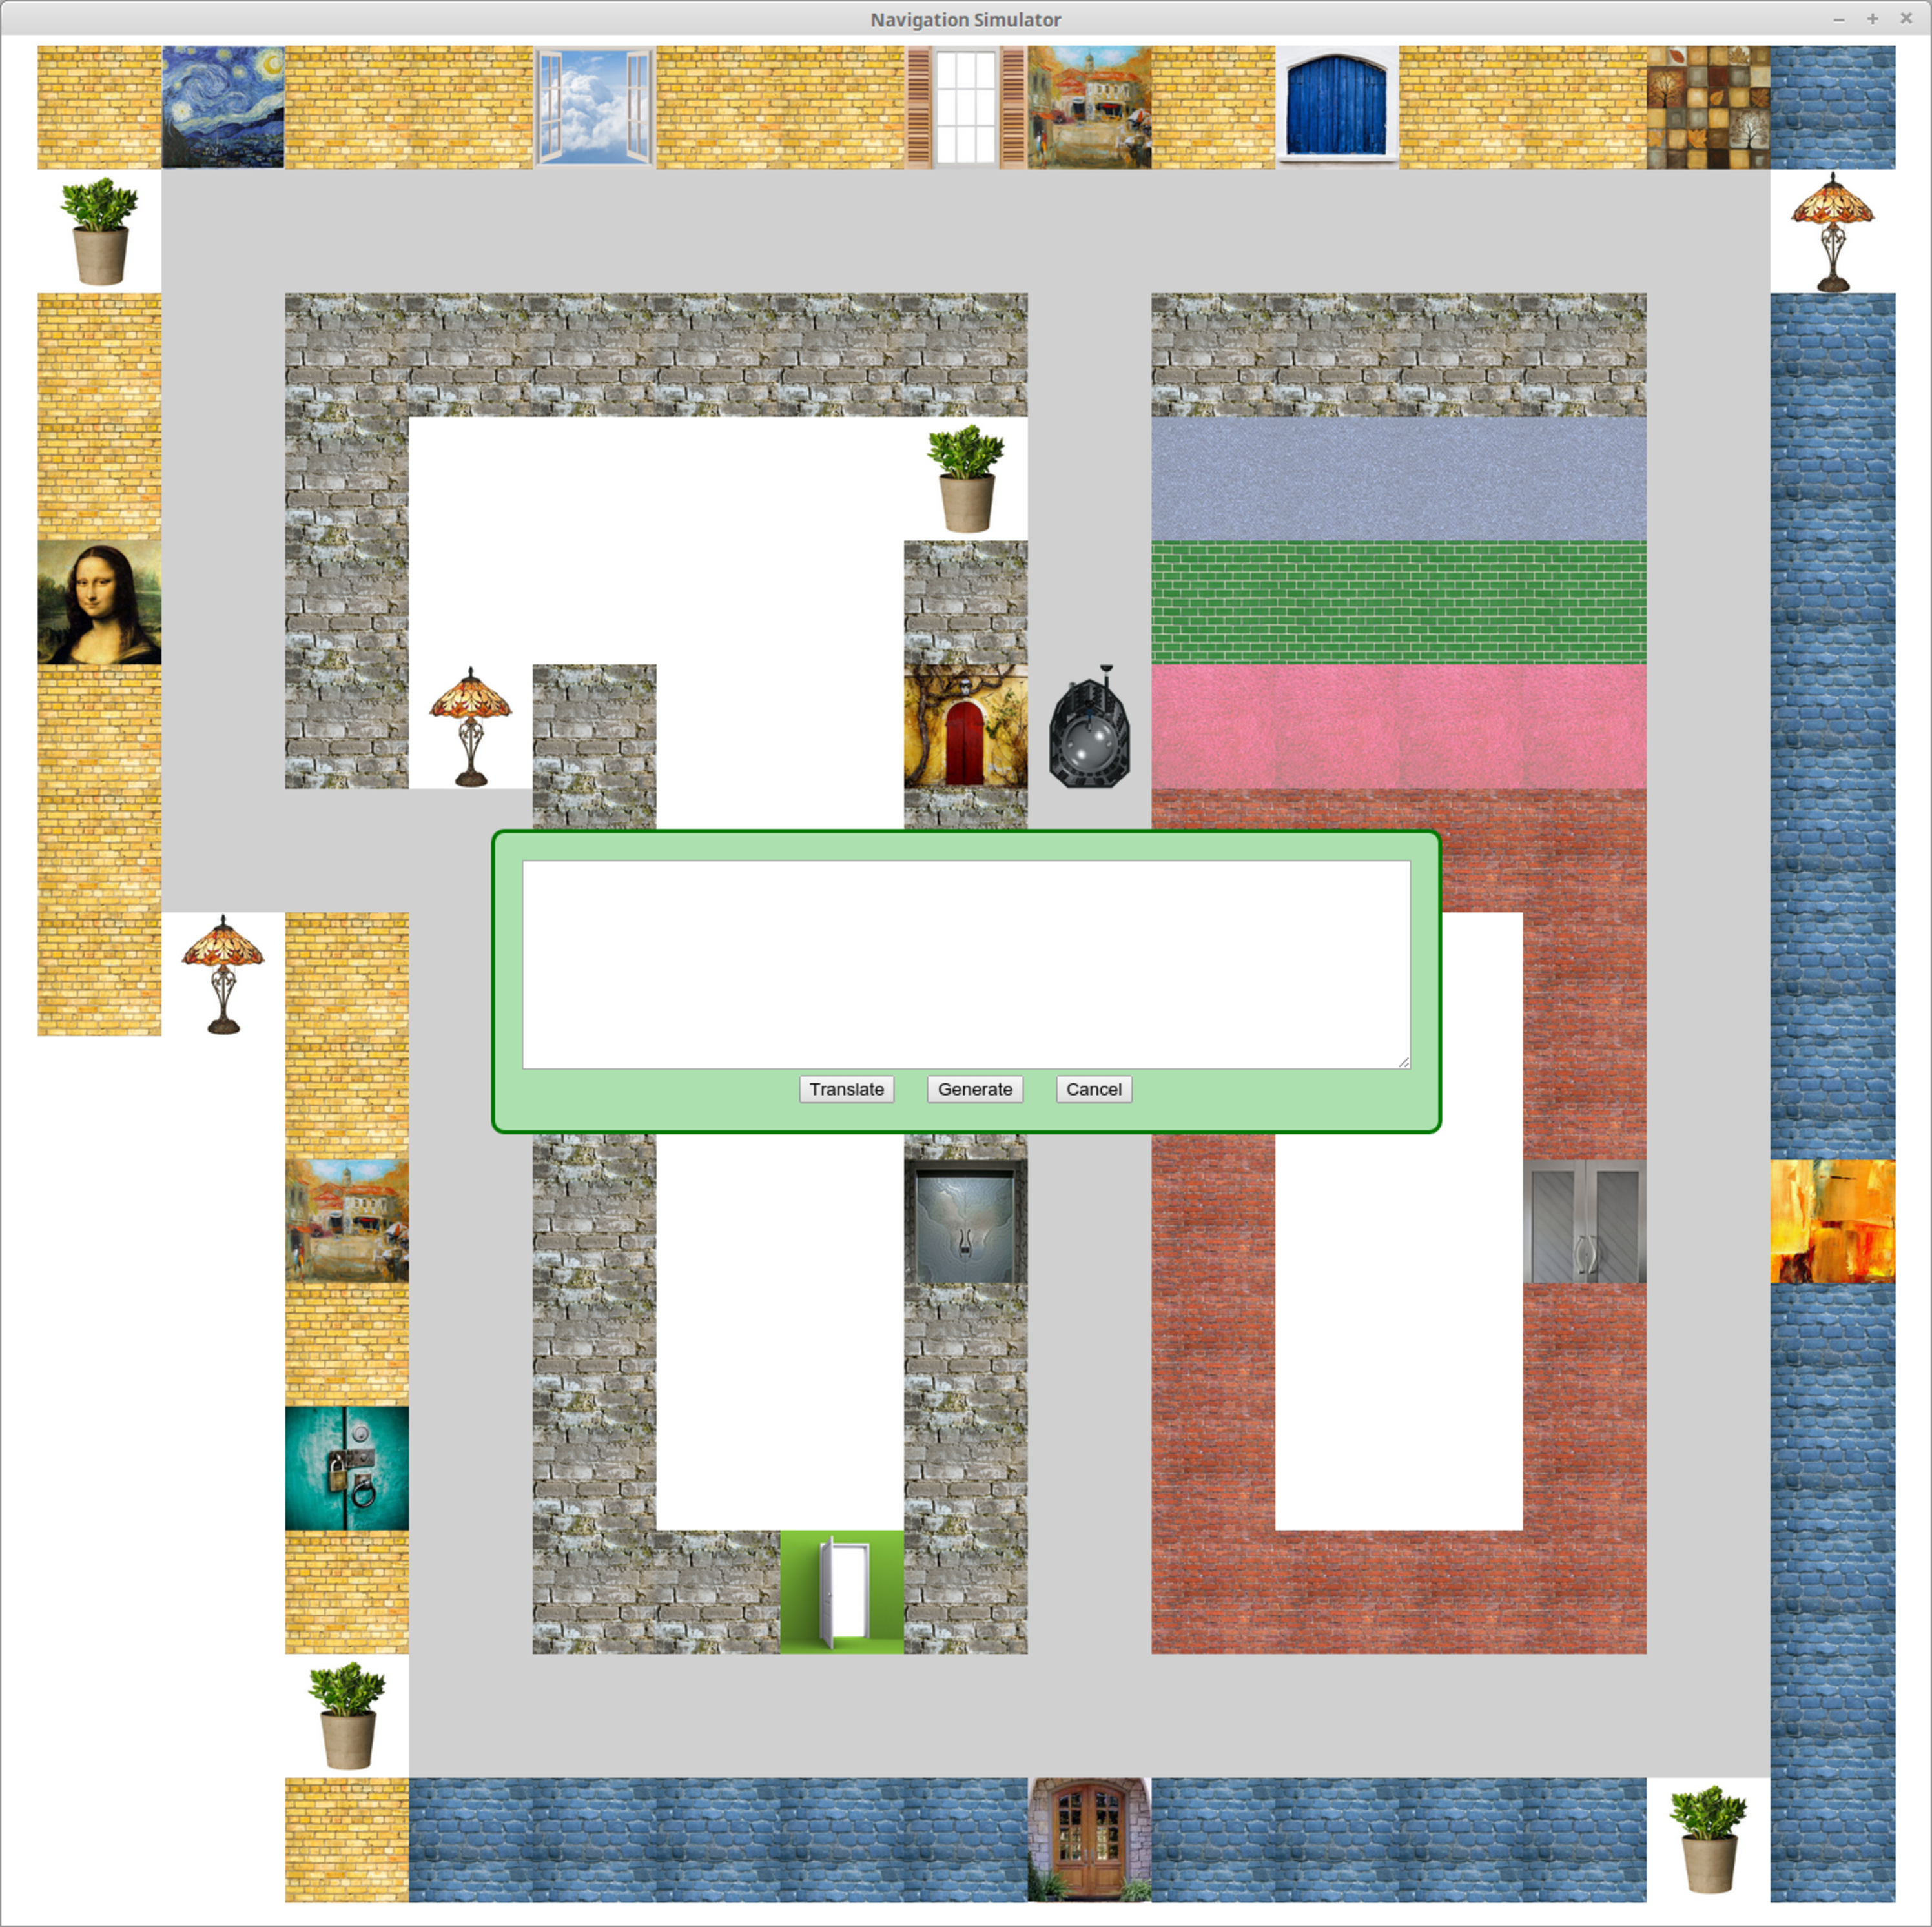
\includegraphics[scale=0.15]{interface.pdf}
\caption{Navigation simulator user interface}\label{fig:interface}
\end{figure}

\begin{figure}[ht!]
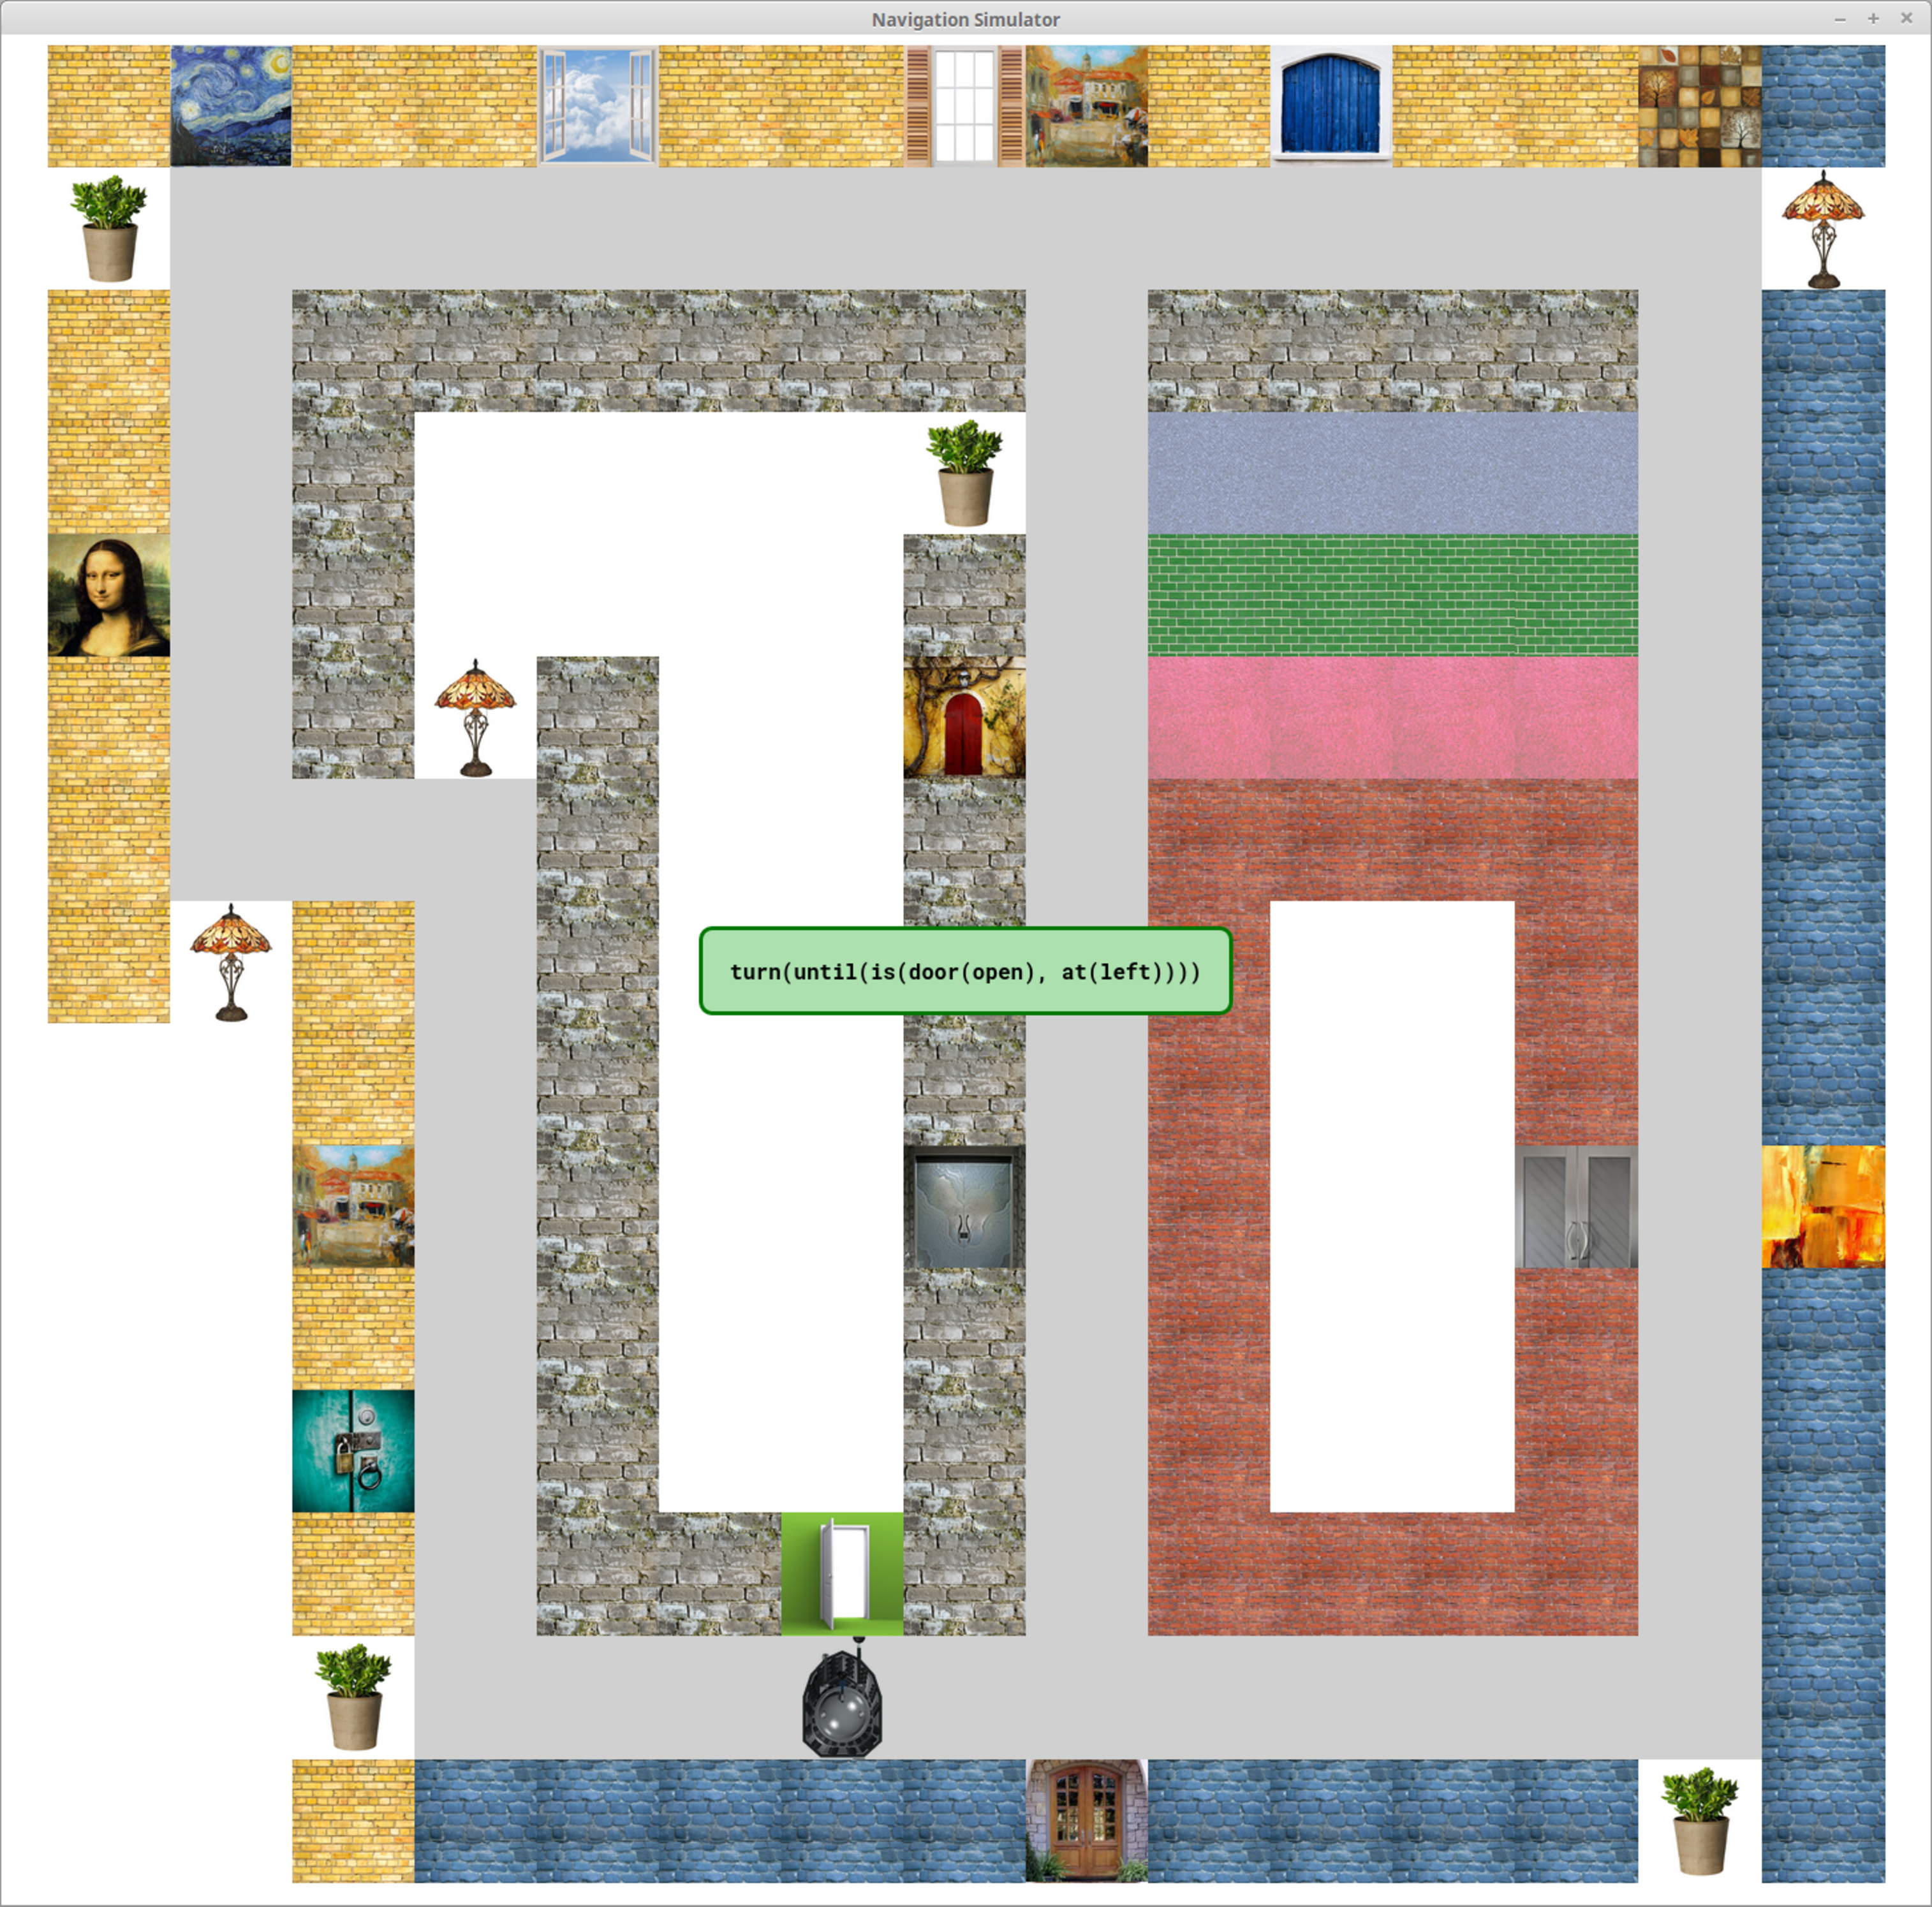
\includegraphics[scale=0.15]{turninst.pdf}
\caption{The robot is presented a turn instruction}\label{fig:turninst}
\end{figure}

\begin{figure}[ht!]
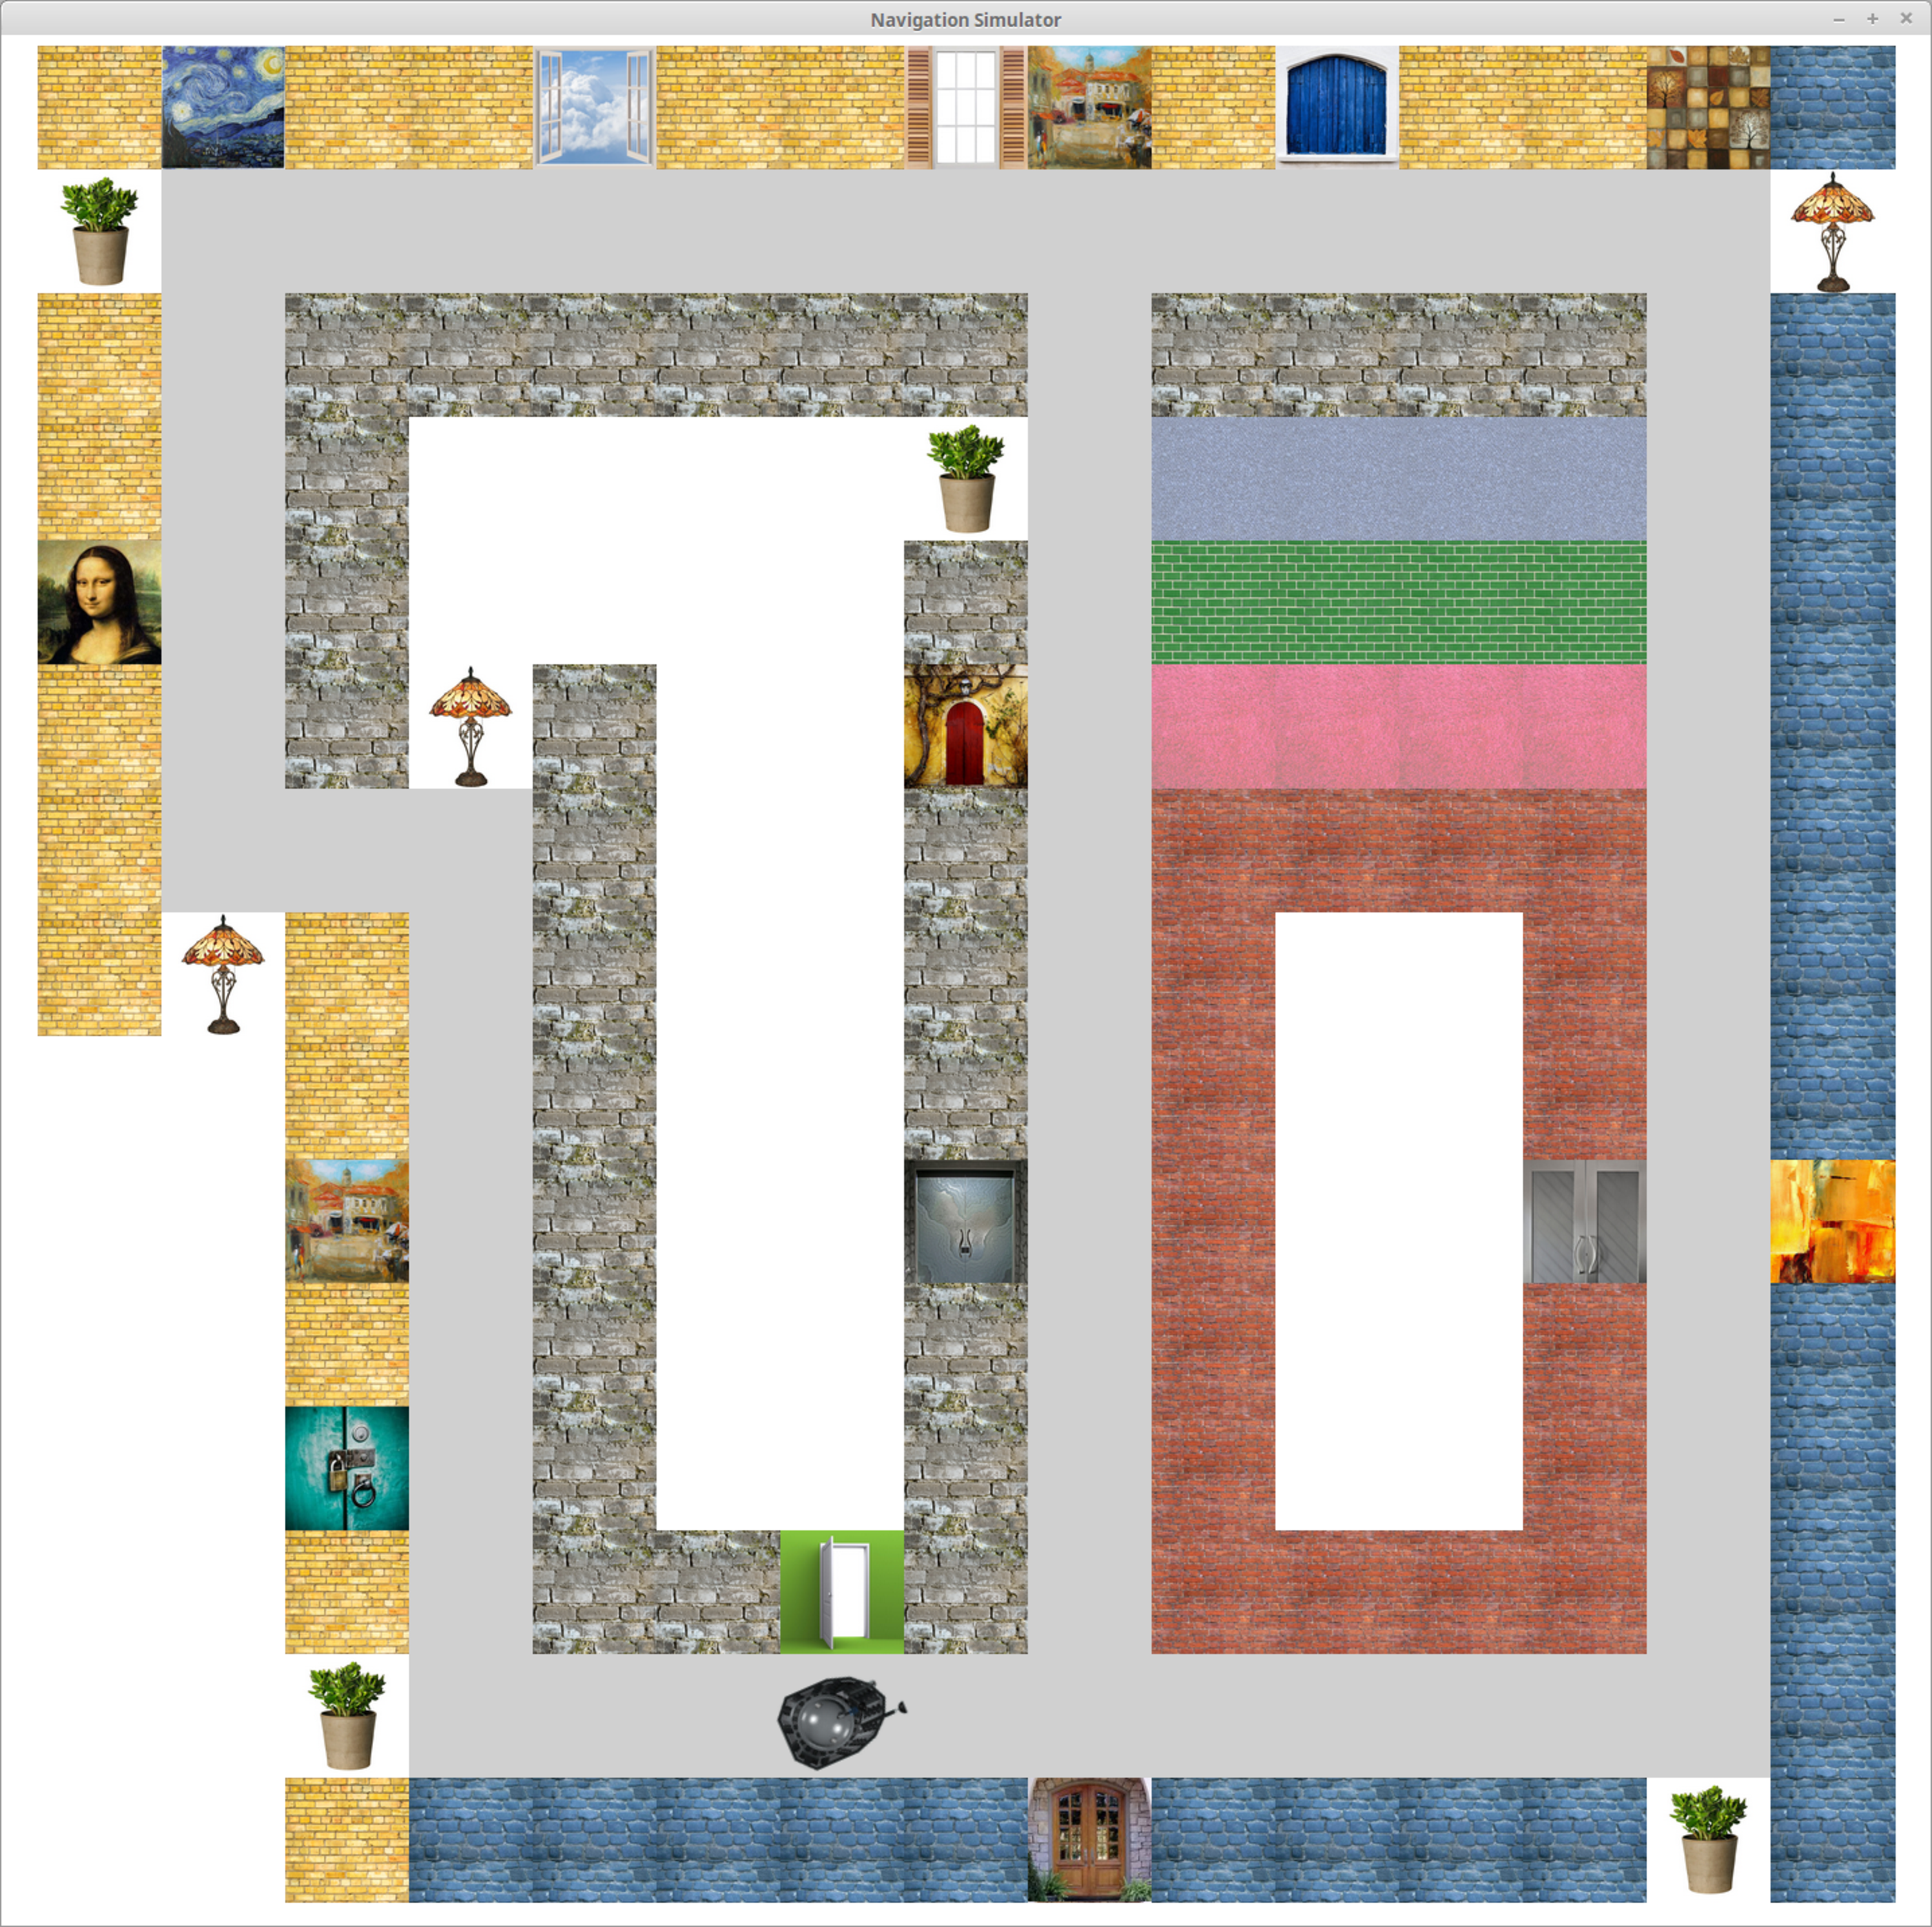
\includegraphics[scale=0.15]{robotturning.pdf}
\caption{Robot in the process of turning}\label{fig:robotturning}
\end{figure}

\begin{figure}[ht!]
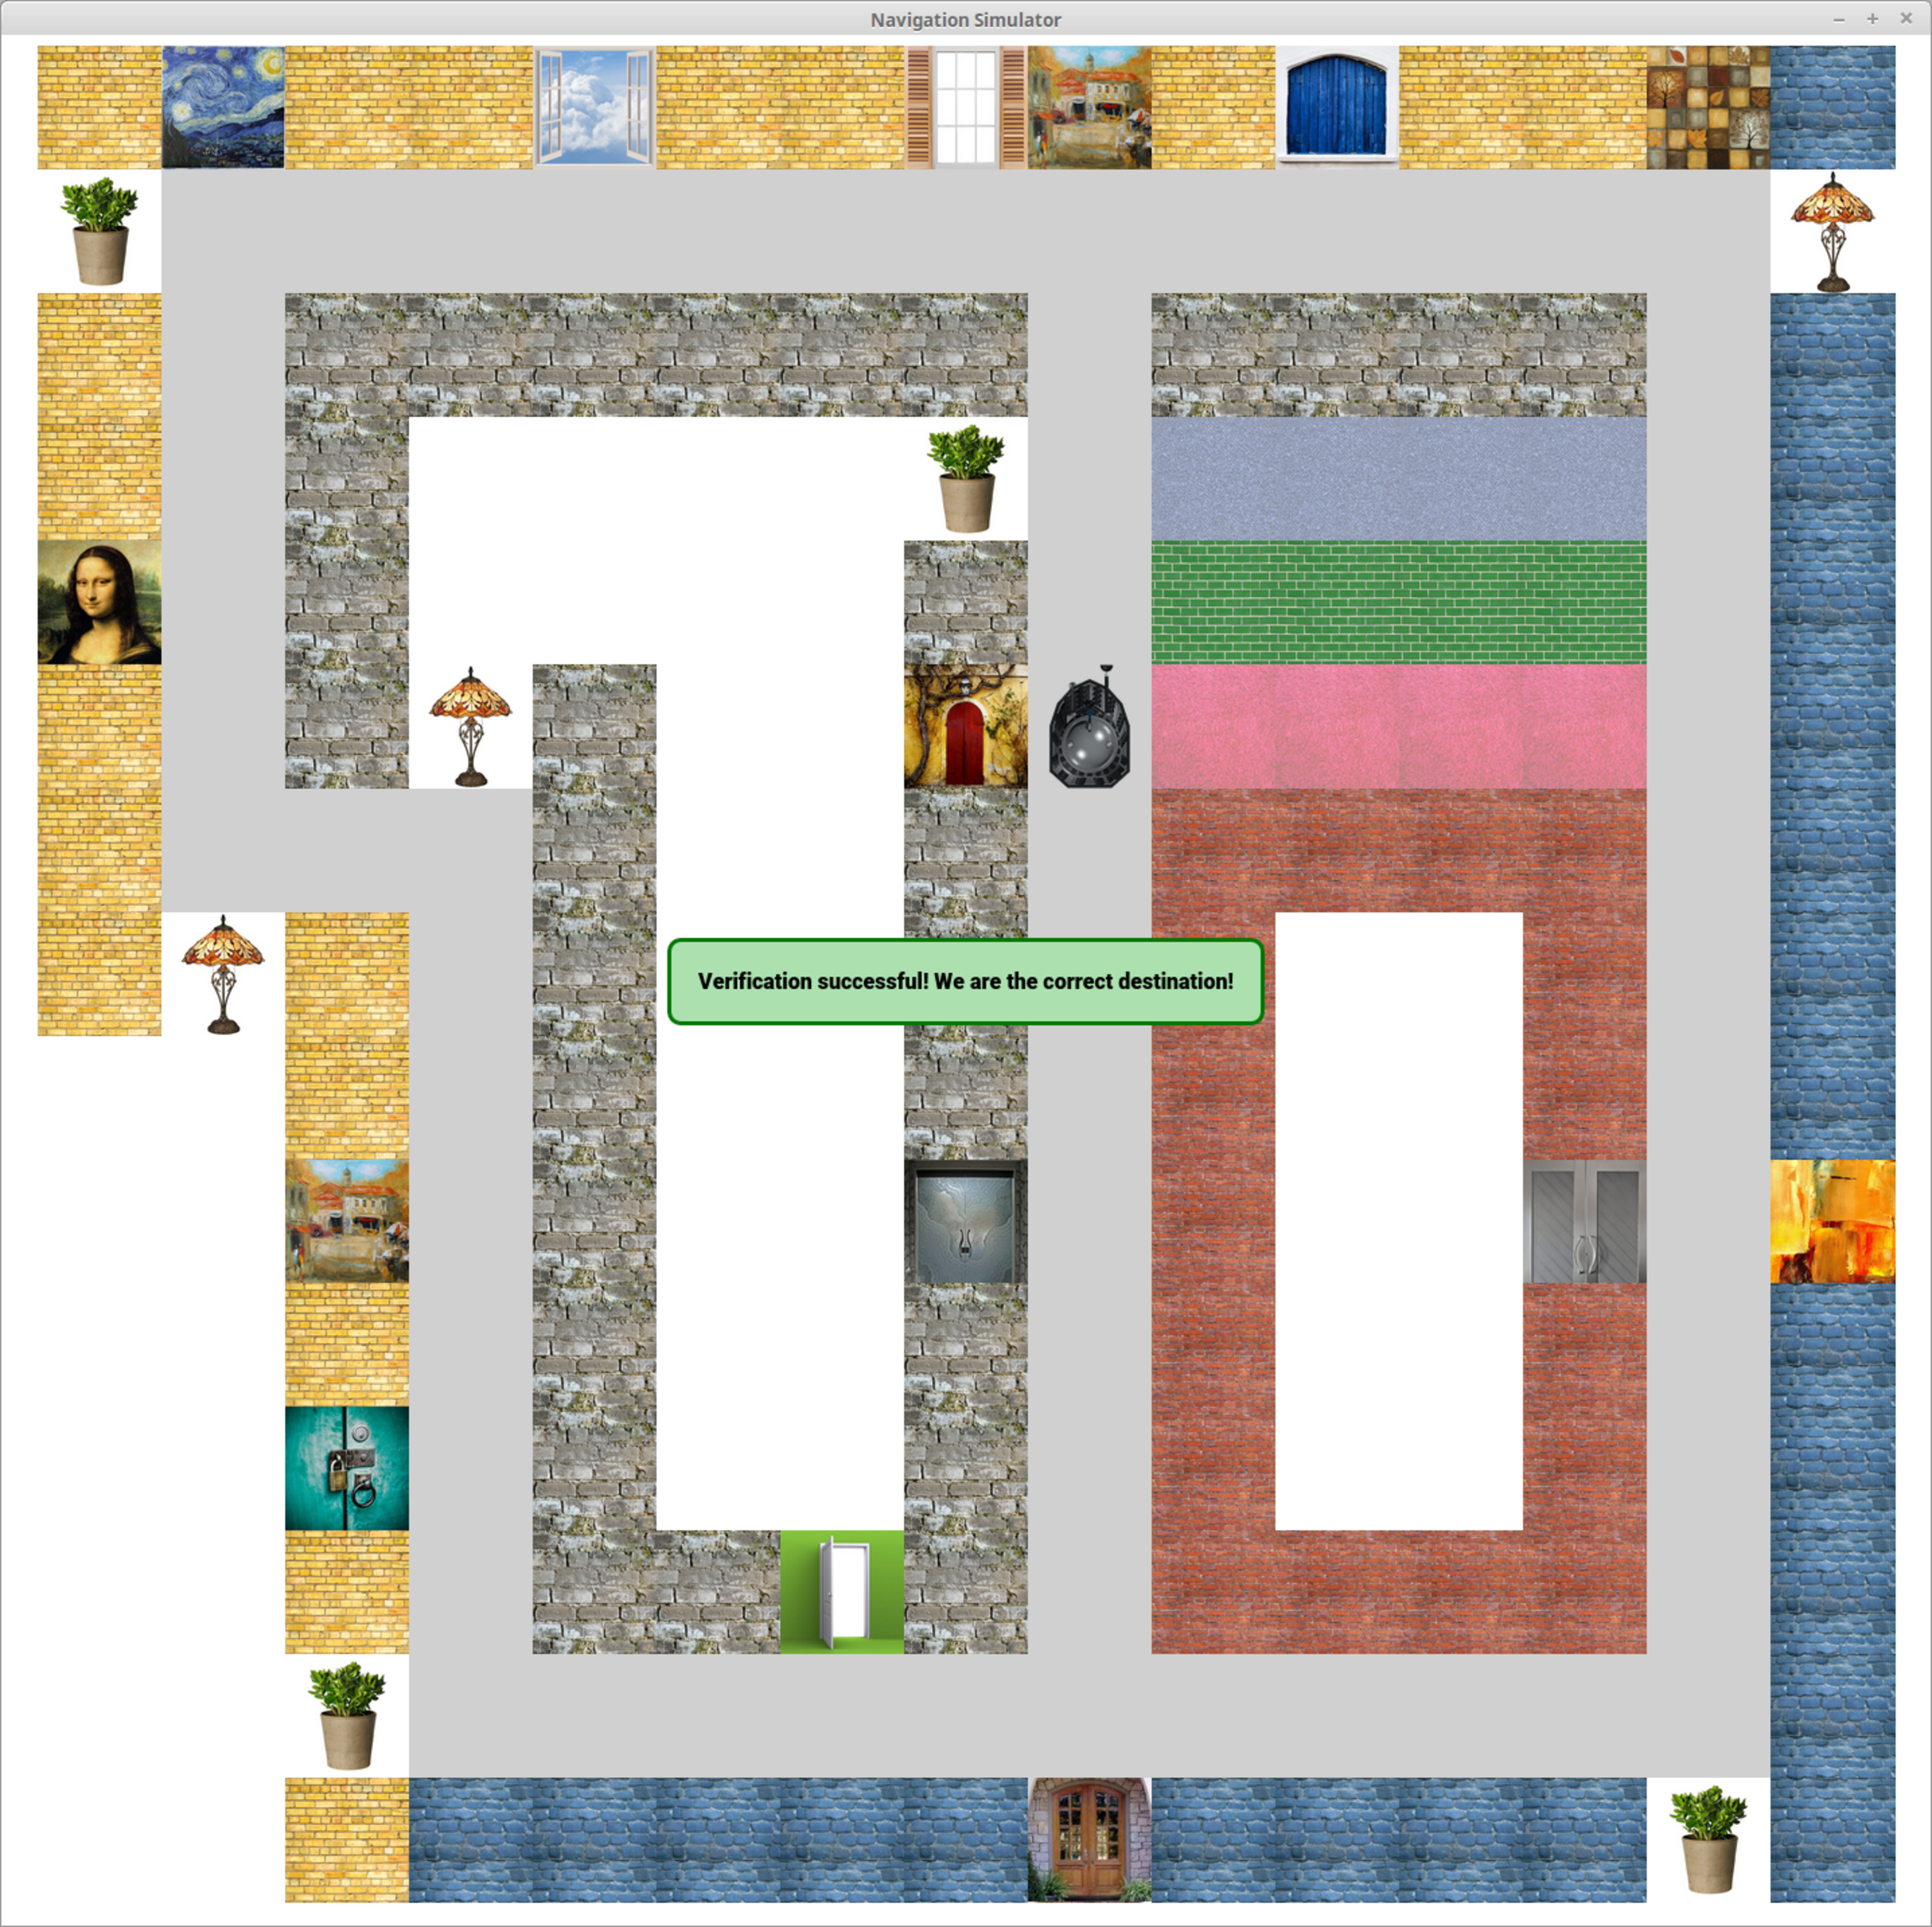
\includegraphics[scale=0.15]{verifysuccess.pdf}
\caption{Successful verification of destination}\label{fig:verifysuccess}
\end{figure}

\begin{figure}[ht!]
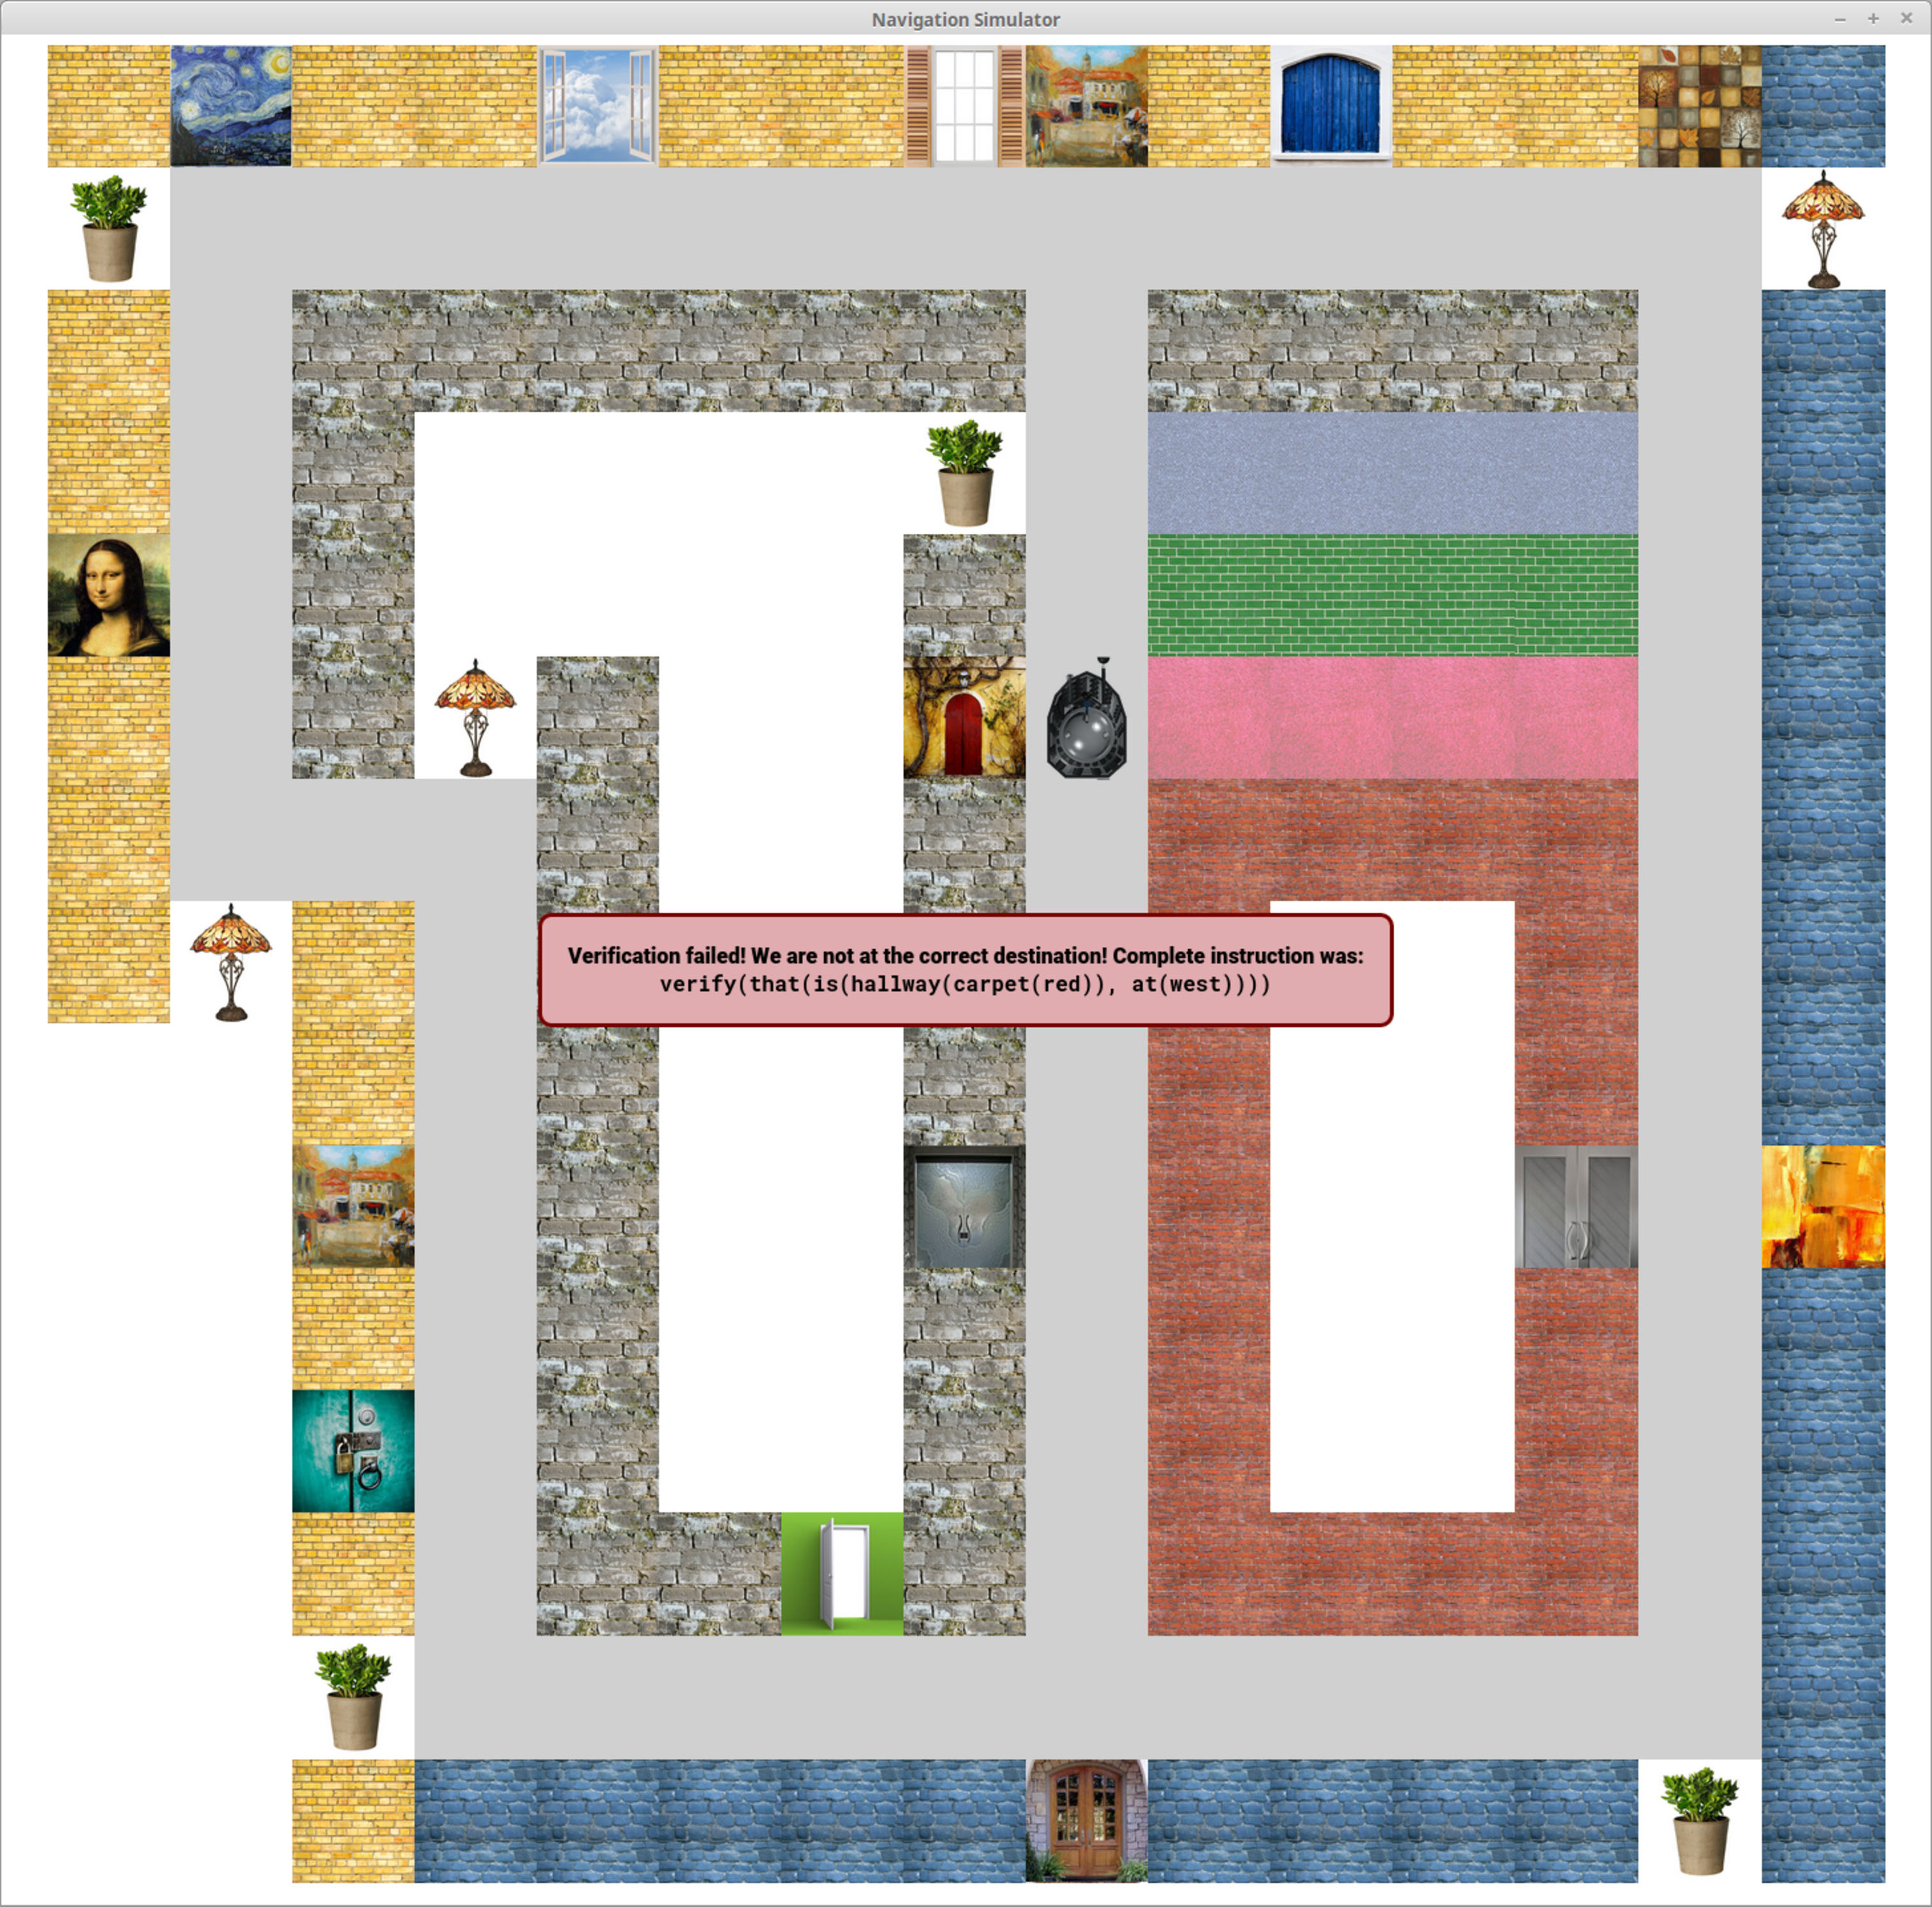
\includegraphics[scale=0.15]{verifyfail.pdf}
\caption{Unsuccessful verification of destination}\label{fig:verifyfail}
\end{figure}

\subsection{Evaluation}

Using the simulator that we created, it was easy for us to verify the accuracy of our translations. However, we still had a problem as far as the amount of test and training data was concerned. As described in \S\ref{ssec:usingnl2kr}, there we some sentence variations that we could not train NL2KR to recognize, which meant that we could not use the complete data set. In addition, the instructions presented in the original data set applied to the simulated world that the authors had created, and as a result, could not be directly applied to our simulation. Our solution to this problem was to automatically generate English sentences and the equivalent formal-representations, out of a randomly-generated path through the simulated world. For the English sentences, we created a template of different variations for each of the different instructions. Using these templates and a randomly-generated path, it was now possible for us to generate large numbers of navigational instructions in English quite quickly. The added advantage was also that we were able to generate the equivalent formal-representation as well, which meant that we could use our generator for both training and testing.

To train the model, we used 70 sentences that cover the different variations of navigational instructions that NL2KR is able to handle. The initial  lexicon that we provided contained 103 meanings, and the trained lexicon contained 251 meanings. To evaluate the trained model, we auto-generated five test sets of 100 sentences and equivalent formal-forms each, and then tested the trained model against each of them. We also evaluated the model by using the simulator, and verified visually whether the translation was correct.

\section{Conclusion and Results}

Against the five auto-generated test-sets of, the model reported an average accuracy of XX\%. Evaluation using the simulator gave similar results as well. In both scenarios, we noticed that the incorrect translation was \textit{syntactically} incorrect, rather than \textit{semantically} incorrect. Hence, we never really encountered a situation where the robot didn't arrive at the correct destination. Instead, the simulator would report parse-errors since the formal form didn't match the grammar that we had defined.

While some inaccuracies are to be expected, we think that it might be possible to improve the performance of the model by training it against a larger data-set so that it can generalize better. However, some of the issues with NL2KR will need to be addressed as well, so that we can provide more-sensible semantics for certain words. We also noticed that both learning and testing seemed to take a very long time. Simply evaluating against the training set of 70 sentences seemed to take at least 20 minutes. We also noticed that this was most prevalent in sentences with complex parse-trees, and also seemed to be affected by the number of overrides in our syntax-override file.

While training and testing, most of our difficulty stemmed from having to define the semantics up-front, which turned out to be a little involved for complicated parse-trees. Artifacts of the lambda-syntax and parsing-logic used by NL2KR also caused us some issues with respect to defining word semantics; we were required to use a form that would work with NL2KR's parser and didn't used any of NL2KR's own tokens from its lambda-grammar. This can be considered a drawback since it limits the expressivity of the translator, and doesn't let us translate natural-sentences into arbitrary formal-representations. However, since the underlying theory is sound, this should only be a matter of making NL2KR's lambda syntax and parser more robust.
\begin{table}[t]
\centering
\resizebox{\columnwidth}{!}{%
\begin{tabular}{|c|c|c|c|c|}
\hline
\rowcolor[HTML]{C0C0C0} 
\textbf{Test Set \#} & \textbf{Sentences} & \textbf{Correct} & \textbf{Incorrect} & \textbf{Accuracy} \\ \hline
1                    & 100                      &                               &                                 &                   \\ \hline
\rowcolor[HTML]{EFEFEF} 
2                    & 100                      &                               &                                 &                   \\ \hline
3                    & 100                      &                               &                                 &                   \\ \hline
\rowcolor[HTML]{EFEFEF} 
4                    & 100                      &                               &                                 &                   \\ \hline
5                    & 100                      &                               &                                 &                   \\ \hline
\end{tabular}
}
\caption{Performance of trained model across 5 test-sets}\label{table:results}
\end{table}
Overall, we feel that using NL2KR is a viable approach for translating natural-languages into formal representations, and also believe that we have amply demonstrated its viability by applying NL2KR successfully in an instance of this particular problem. 


\bibliography{nlp-navigation}
\bibliographystyle{naaclhlt2016}


\end{document}
